\documentclass[0-protokol.tex]{subfiles}
\begin{document}

\subsection*{Úkol 1}
Pomocí zapojení \ref{fig:zap_u1} jsem na osciloskopu odečetl špičkové napětí $U_{0, osc} = \SI{10,8 \pm 0,2}{V}$ při nastaveném rozsahu $\SI{2}{V}$. Za chybu jsem určil polovinu nejmenšího dílku stupnice.

Na digitálním multimetru, nastaveného na rozsah $\SI{20}{V}$ střídavého napětí, jsem změřil efektivní hodnotu napětí $\SI{7,67 \pm 0,06}{V}$, což po přepočtu podle vzorce \eqref{eq:ef_napeti} dá špičkovou hodnotu napětí $U_{0, mm} = \SI{10,85 \pm 0,08}{\volt}$.

\subsection*{Úkol 2}
V následující tabulce uvádím naměřené hodnoty pro úkol 2a pomocí zapojení \ref{fig:zapojeni_filtrace} (bez ampérmetru). Chyba kapacity byla určena jako $\SI{1}{\percent}$ z hodnoty, nastavené na kapacitní dekádě, chyba napětí byla určena odhadem, jelikož hodnota, zobrazovaná multimetrem, se chaoticky měnila v menším či větším okolí uvedených hodnot.
\begin{table}[H] 
\centering
\setlength{\tabcolsep}{15pt}
        \begin{tabular}{cccc}                                        \toprule
        {C}          &      {$\sigma_C$} & {U}          & {$\sigma_U$} \\ 
        {$[\si{F}]$} &      {$[\si{F}]$} & {$[\si{V}]$} & {$[\si{V}]$} \\ \midrule
   \num{1e-10}       & \num{1e-12}       & 3,3          & 0,2          \\ 
   \num{1e-08}       & \num{1e-10}       & 3,3          & 0,2          \\ 
   \num{2e-08}       & \num{2e-10}       & 3,5          & 0,2          \\ 
   \num{3e-08}       & \num{3e-10}       & 3,9          & 0,2          \\ 
   \num{4e-08}       & \num{4e-10}       & 4,2          & 0,3          \\ 
   \num{5e-08}       & \num{5e-10}       & 4,5          & 0,3          \\ 
   \num{6e-08}       & \num{6e-10}       & 4,9          & 0,3          \\ 
   \num{7e-08}       & \num{7e-10}       & 5,2          & 0,3          \\ 
   \num{8e-08}       & \num{8e-10}       & 5,3          & 0,3          \\ 
   \num{9e-08}       & \num{9e-10}       & 5,7          & 0,3          \\ 
   \num{1e-07}       & \num{1e-09}       & 5,9          & 0,3          \\ 
   \num{2e-07}       & \num{2e-09}       & 7,3          & 0,3          \\ 
   \num{3e-07}       & \num{3e-09}       & 7,9          & 0,3          \\ 
   \num{5e-07}       & \num{5e-09}       & 8,6          & 0,3          \\ 
   \num{7e-07}       & \num{7e-09}       & 8,9          & 0,2          \\ 
   \num{1e-06}       & \num{1e-08}       & 9,2          & 0,2          \\ 
   \num{2e-06}       & \num{2e-08}       & 9,6          & 0,2          \\ 
   \num{3e-06}       & \num{3e-08}       & 9,7          & 0,1          \\ 
   \num{4e-06}       & \num{4e-08}       & 9,8          & 0,1          \\ 
   \num{5e-06}       & \num{5e-08}       & 9,8          & 0,1          \\ 
   \num{6e-06}       & \num{6e-08}       & 9,8          & 0,1          \\ 
   \num{7e-06}       & \num{7e-08}       & 9,8          & 0,1          \\ 
   \num{8e-06}       & \num{8e-08}       & 9,9          & 0,1          \\ 
   \num{9e-06}       & \num{9e-08}       & 9,9          & 0,1          \\ 
   \num{1e-05}       & \num{1e-07}       & 9,9          & 0,1          \\ \bottomrule

\end{tabular}
\caption{Naměřené hodnoty pro úkol 2a}
\label{tab:u2a}
\end{table}

Průběh závislosti stejnosměrné složky napětí na filtrační kapacitě uvádím v následujícím grafu.
\begin{figure}[H]
\centering
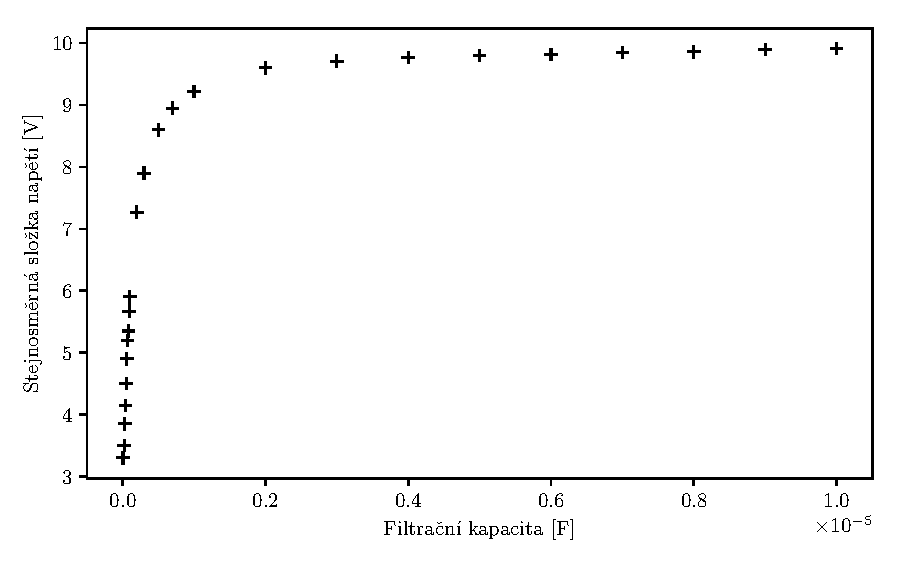
\includegraphics[]{u2a}
\caption{Závislost stejnosměrného napětí na filtrační kapacitě}
\label{fig:u2a}
\end{figure}

Následující tabulka obsahuje hodnoty, naměřené pro úkol 2b pomocí zapojení \ref{fig:zapojeni_filtrace}. Chyby byly určeny shodně s předešlým případem.
\begin{table}[H] 
\centering
\setlength{\tabcolsep}{15pt}
\begin{tabular}{cccc}                                                \toprule
$I_{st}$      & $\sigma_{I_{st}}$ & $C$           & $\sigma_C$    \\ 
$[\si{A}]$    & $[\si{A}]$        & $[\si{F}]$    & $[\si{F}]$    \\ \midrule
\num{9.5e-05} & \num{1e-05}       & \num{1.5e-06} & \num{1.5e-08} \\ 
\num{1.1e-04} & \num{1e-05}       & \num{1.7e-06} & \num{1.7e-08} \\ 
\num{1.2e-04} & \num{1e-05}       & \num{1.9e-06} & \num{1.9e-08} \\ 
\num{1.4e-04} & \num{1e-05}       & \num{2.1e-06} & \num{2.1e-08} \\ 
\num{1.5e-04} & \num{1e-05}       & \num{2.4e-06} & \num{2.4e-08} \\ 
\num{1.9e-04} & \num{1e-05}       & \num{2.9e-06} & \num{2.9e-08} \\ 
\num{2.3e-04} & \num{1e-05}       & \num{3.6e-06} & \num{3.6e-08} \\ 
\num{3.1e-04} & \num{1e-05}       & \num{4.8e-06} & \num{4.8e-08} \\ 
\num{4.5e-04} & \num{1e-05}       & \num{7.1e-06} & \num{7.1e-08} \\ 
\num{5.6e-04} & \num{1e-05}       & \num{9.2e-06} & \num{9.2e-08} \\ \bottomrule

\end{tabular}
\caption{Naměřené hodnoty pro úkol 2b}
\label{tab:u2b}
\end{table}

Lineární závislost filtrační kapacity na protékaném proudu je vyobrazena v následujícím grafu. Protože relativní chyby proudu jsou mnohem významnější než chyby kapacity, graf obsahuje horizontální chybové úsečky.
\begin{figure}[H]
\centering
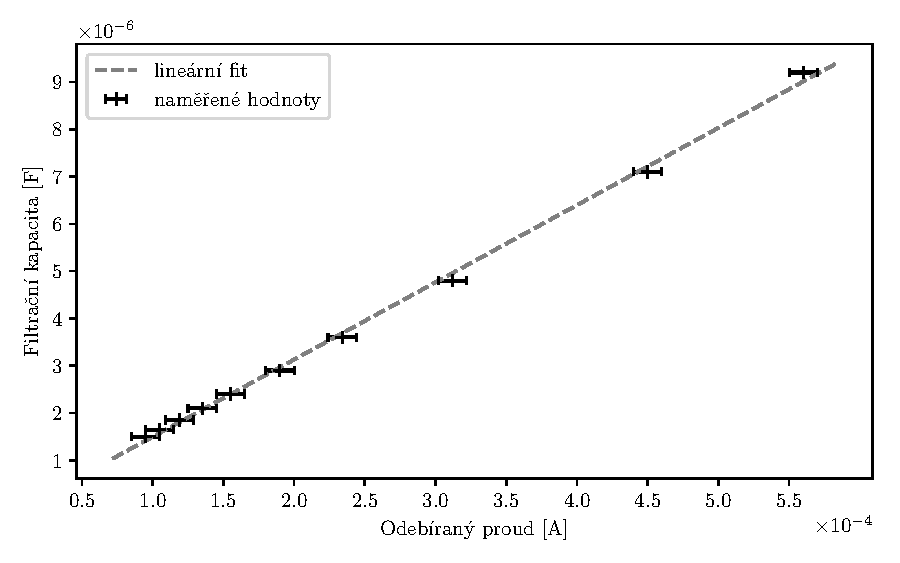
\includegraphics[]{u2b}
\caption{Závislost filtrační kapacity na protékaném proudu}
\label{fig:u2b}
\end{figure}

\subsection*{Úkol 3}
S pomocí zapojení \ref{fig:volt-amper} jsem při sledování volt-ampérové charakteristiky z displeje osciloskopu odečetl proud při nulovém napětí $I_{U=\SI{0}{V}} = \SI{1 \pm 0,05}{mA}$ a napětí při proudu $\SI{20}{mA}$ $U_{A=\SI{20}{mA}} = \SI{5,2 \pm 0,2}{V}$. Tyto hodnoty jsou také zakresleny v přiloženém obrázku 9.

Při měření Zenerovy diody jsem odečetl napětí při proudu $\SI{20}{mA}$ $U_{A=\SI{20}{mA}} = \SI{0,7 \pm 0,03}{V}$ a Zenerovo napětí $U_{Zener} = \SI{-6,6 \pm 0,03}{V}$. Tyto hodnoty jsou zakresleny v přiloženém obrázku 10.

Všechny uvedené chyby byly určeny velikostí nejmenšího dílku stupnice osciloskopu na rozdíl od úkolu 1, kde jsem použil polovinu nejmenšího dílku. Může za to fakt, že tělo osciloskopu bylo patrně mírně zmagnetováno a volt-ampérová charakteristika byla mírně zdvojena. 

\end{document}
